%%%%%%%%%%%%%%%%%%%%%%%%%%%%%%%%%%%%%%%%%
% Long Professional Curriculum Vitae
% LaTeX Template
% Version 1.1 (9/12/12)
%
% This template has been downloaded from:
% http://www.latextemplates.com
%
% Original author:
% Rensselaer Polytechnic Institute (http://www.rpi.edu/dept/arc/training/latex/resumes/)
%
% Important note:
% This template requires the res.cls file to be in the same directory as the
% .tex file. The res.cls file provides the resume style used for structuring the
% document.
%
%%%%%%%%%%%%%%%%%%%%%%%%%%%%%%%%%%%%%%%%%

%----------------------------------------------------------------------------------------
% PACKAGES AND OTHER DOCUMENT CONFIGURATIONS
%----------------------------------------------------------------------------------------

\let\nofiles\relax
\documentclass{res}[12pt] % Use the res.cls style, the font size can be changed to 11pt or 12pt here
%\usepackage{helvet}
%\renewcommand{\familydefault}{\sfdefault}
%\usepackage{CormorantGaramond}
\usepackage{fontspec}
\setmainfont{Avenir Next}[BoldFont={Avenir Next Demi Bold}]
\usepackage{fontmfizz}

\usepackage{fontawesome5}

\usepackage{graphicx}
\usepackage[official]{eurosym}
\usepackage{wrapfig}
\usepackage[hidelinks]{hyperref}
\usepackage{caption}
\captionsetup[figure]{labelformat=empty}

%\usepackage[style=numeric,sorting=ydnt,defernumbers,maxbibnames=20]{biblatex}
% \addbibresource{publications.bib}
%\AtEveryBibitem{\clearfield{url}}

\newcommand{\rEntry}[1]{\textbf{ #1}}
\newcommand{\rSection}[1]{\section{\Large\centerline{#1}}}
\newcommand{\sectionRule}{{\vspace{-6pt} \color{black} \hrulefill}}

\usepackage{xcolor}
% Define colors for social media links
\definecolor{email}{RGB}{0, 0, 0}
\definecolor{github}{RGB}{36, 41, 46}
\definecolor{youtube}{RGB}{255, 0, 0}
\definecolor{linkedin}{RGB}{0, 119, 181}

% Change hyperlink colors to remove ugly boxes
\hypersetup{
    colorlinks,
    linkcolor={blue!80!black},
    citecolor={blue!80!black},
    urlcolor={blue!80!black}
}

\usepackage{longtable}
\usepackage{tikz}
\usepackage{multicol}
\usepackage{emoji}


\usetikzlibrary{shapes.misc}

\definecolor{skillbg}{HTML}{CCCCCC}
\definecolor{skillbar1}{HTML}{333333}
\definecolor{skillbar2}{HTML}{555555}
\definecolor{skillbar3}{HTML}{777777}
\definecolor{skillbar4}{HTML}{999999}
\definecolor{skillbar5}{HTML}{BBBBBB}

\newcommand{\skillbar}[1]{%
  \begin{tikzpicture}[scale=0.5, transform shape, rounded rectangle west arc=0pt, rounded rectangle east arc=0pt, minimum width=5mm, minimum height=2mm]
    \foreach \x in {1,2,3,4,5}{
      \ifnum\x>#1
        \fill [color=skillbg] (\x-1,0) rectangle (\x,0.4);
      \else
        \fill [color=skillbar\x] (\x-1,0) rectangle (\x,0.4);
      \fi
      \draw [color=skillbar\x, fill=none, line width=1pt, rounded corners=2pt] (\x-1,0) rectangle (\x,0.4);
      \ifnum\x<5
        \draw [color=skillbg, line width=0.5pt] (\x,0) -- (\x,0.4);
      \fi
    }
  \end{tikzpicture}
}

\newsectionwidth{0pt} % Stops section indenting\

\pagestyle{plain}

\begin{document}

%----------------------------------------------------------------------------------------
% YOUR NAME AND ADDRESS(ES) SECTION
%----------------------------------------------------------------------------------------

\begin{figure}[htbp]
\begin{center}
%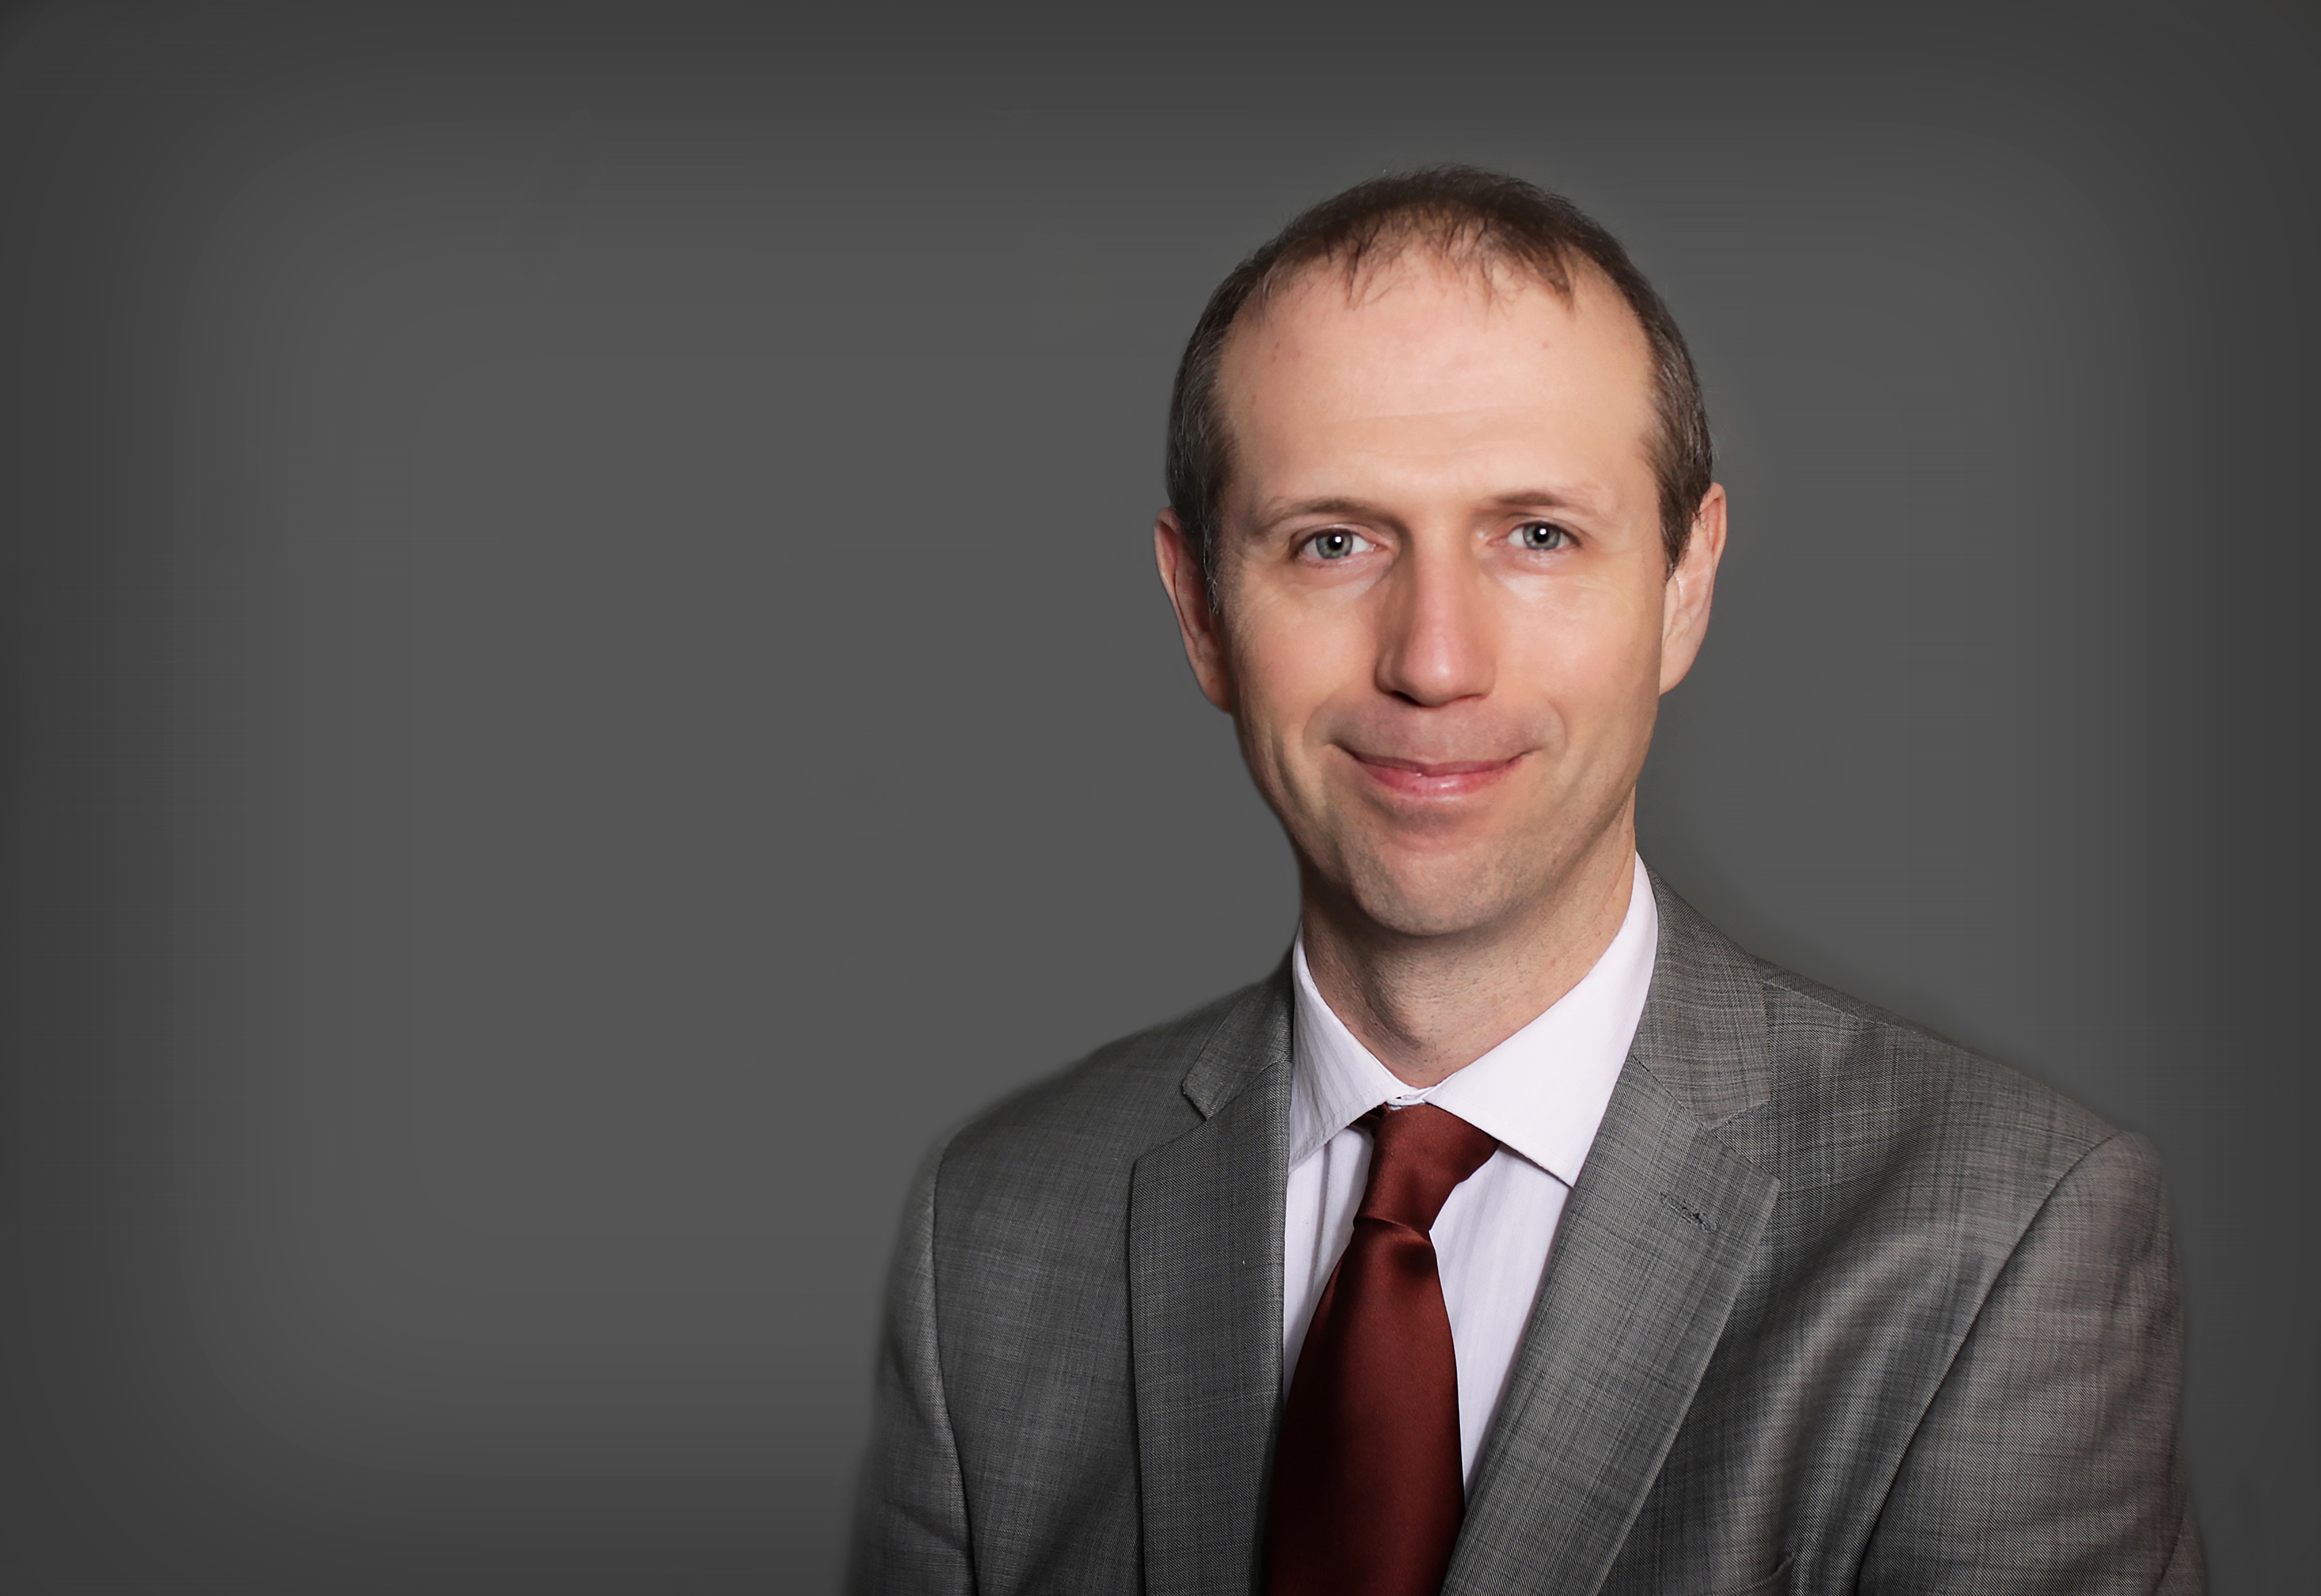
\includegraphics[width=0.125\textwidth]{figures/John.jpg}
\end{center}
\end{figure}

\name{Jacopo Uggeri} % Your name at the top

% If you don't want one of the addresses, simply remove all the text in the first or second \address{} bracket

\address{{\bf Address} \\ 134-136 Cromwell Road \\ SW74HA \\ London \\ United Kingdom} % Your address 1

\address{{\bf Contact} \\
\href{mailto:jacopo.uggeri@gmail.com}{\textcolor{email}{jacopo.uggeri@gmail.com}} \\
\href{https://github.com/jacopouggeri}{\textcolor{github}{\faGithub\ GitHub}} \\
\href{https://www.youtube.com/c/jacopouggeri}{\textcolor{youtube}{\faYoutube\ YouTube}} \\
\href{https://www.linkedin.com/in/jacopo-uggeri-191}{\textcolor{linkedin}{\faLinkedin\ LinkedIn}}}



%----------------------------------------------------------------------------------------

\begin{resume}

%----------------------------------------------------------------------------------------
% OBJECTIVE SECTION
%----------------------------------------------------------------------------------------

\rSection{Summary}
\sectionRule
\vspace{6pt} % Gap between title and text

%----------------------------------------------------------------------------------------
% PROFESSIONAL EXPERIENCE SECTION
%----------------------------------------------------------------------------------------

\rSection{Professional Experience}
\sectionRule
\vspace{6pt} % Gap between title and text

% \begin{itemize} \itemsep -2pt % Reduce space between items
% \end{itemize}

\rEntry{Graduate Teaching Assistant} \\
Department of Physics, Imperial College London (London), United Kingdom \hfill 2022 -- 2023

%----------------------------------------------------------------------------------------

% \vspace{0.2in} % Some whitespace between sections

%----------------------------------------------------------------------------------------
% EDUCATION SECTION
%----------------------------------------------------------------------------------------

\rSection{Education}
\sectionRule
\vspace{6pt} % Gap between title and text

\rEntry{ MSci Physics with Theoretical Physics}\\ 
Imperial College London (London), United Kingdom \hfill 2019 -- present

\begin{itemize} \itemsep -2pt
\item Undergraduate Integrated Masters programme in physics, attended a variety of courses that granted a solid foundation in scientific and critical thinking, with a focus on theoretical physics
\item Excellent academic performance, achieved 1st in theoretical modules: Mathematical Methods, Foundations of Quantum Mechanics, Advanced Classical Physics, Group Theory, Nuclear and Particle Physics, Statistical Mechanics
\item Current relevant courses: Quantum Field Theory, Unification, General Relativity, Cosmology
\item Used Python extensively for data analysis of experiments and simulations
\end{itemize}

\rEntry{ Diploma di Liceo Scientifico Tradizionale}\\ 
Liceo Scientifico Giovanni Gandini (Lodi), Italy \hfill 2013 -- 2019

\begin{itemize} \itemsep -2pt
\item A scientifically oriented high school with a wide range of subjects spanning both sciences and humanities
\item Participated in extracurricular events and activities with a focus on Physics and Mathematics
\item Graduated with 100/100 at \sl{Esame di Stato}
\end{itemize}


%----------------------------------------------------------------------------------------
 
% \vspace{0.2in} % Some whitespace between sections

%----------------------------------------------------------------------------------------
% PROJECTS SECTION
%----------------------------------------------------------------------------------------

\rSection{Projects}
\sectionRule
\vspace{6pt} % Gap between title and text

\rEntry{ Can photo evaporation explain lack of red giants in the galactic centre?}\\ MSci Project at Imperial College London \hfill 2022 -- now
\begin{itemize}
\item The project aims to determine the photo evaporation rate of red giants around supermassive black holes and determine how this phenomenon affects their evolution, to investigate whether it can explain the observed lack of red giants in the galactic centre compared to equilibrium theoretical predictions.
\item Computational and theoretical project: involved writing, testing and organizing code that could be shared with others
\item Helped develop critical scientific thinking and research skills
\end{itemize}

\rEntry{ Search for beyond SM physics from LHCb data}\\ Group Project at Imperial College London \hfill 2021
\begin{itemize}
\item Involved coordinating with other ~20 students to analyze data from LHCb experiment
\item Participated in group discussions and contributed meaningful ideas
\item Main role was to train a machine learning decision tree model to separate background from signal
\end{itemize}


\rEntry{ Improving people counter image recognition neural network} \\ Summer work experience at GrottiniLab with Politecnico di Ancona \hfill 2020 \\ \href{https://github.com/jacopouggeri/curriculumVitae/blob/84ad9712112b11ea237b126a98ba1764b27054b4/attachments/grottini.pdf}{See Attachment}
\begin{itemize}
\item Assigned to a software engineer working on a people counter neural network, with the aim of exploring new avenues of improvement
\item Reviewed literature on the current state of the art of image recognition neural networks
\item Proposed and coded a new data augmentation strategy to improve the people counter
\end{itemize}

\rEntry{ Critical Temperature of an Ising Model on a Sierpinski Gasket} \\ Year 1 Summer Project at Imperial College London  \hfill 2020
\begin{itemize}
\item Worked remotely with a peer to simulate an Ising model on a Sierpinski gasket network
\item Wrote Python code to run, visualize and analyze the simulation, and numerically evaluated the model’s critical temperature and the corresponding critical exponent.
\item Delivered a video summary of the project and a detailed report
\end{itemize}


%----------------------------------------------------------------------------------------
 
% \vspace{0.2in} % Some whitespace between sections

%----------------------------------------------------------------------------------------
% EXPERIENCES SECTION
%----------------------------------------------------------------------------------------

\rSection{Experiences}
\sectionRule
\vspace{6pt} % Gap between title and text

\rEntry{ DeepLearn Summer School} \\ 4th International School on Deep Learning \hfill 2021 \\ \href{https://github.com/jacopouggeri/curriculumVitae/blob/84ad9712112b11ea237b126a98ba1764b27054b4/attachments/deeplearn.pdf}{See Attachment}
\begin{itemize}
\item Attended 38 hours of postgraduate level lectures given by Machine Learning experts from various fields
\item Learned to comprehend and acquire meaningful information from lectures that assumed more advanced background knowledge than I had
\end{itemize}

\rEntry{ Project Extreme Energy Events (EEE)} \\ Long running project organized by INFN involving multiple Italian high schools \hfill 2013 -- 2019
\begin{itemize}
\item Participated in the data taking and analysis process for a MRPC muon detector
\item Attended lectures on particle physics and cosmic rays
\item Participated in joint conferences between participating schools summarizing recent results
\end{itemize}

\rEntry{ Building an MRPC muon detector chamber at CERN } \hfill 2017 \\ \href{https://github.com/jacopouggeri/curriculumVitae/blob/84ad9712112b11ea237b126a98ba1764b27054b4/attachments/eee.pdf}{See Attachment}
\begin{itemize}
\item Worked with peers in a laboratory to assemble a muon detector chamber
\item Attended various seminars hosted by CERN personnel regarding the current state of particle physics
\end{itemize}

%----------------------------------------------------------------------------------------
 
% \vspace{0.2in} % Some whitespace between sections

%----------------------------------------------------------------------------------------
% SKILLS SECTION
%----------------------------------------------------------------------------------------

\rSection{Skills}
\sectionRule
\vspace{6pt} % Gap between title and text

\subsection*{Coding}

\begin{multicols}{2}
\begin{itemize}
    \item[\mfPython] Python \hfill\skillbar{0.9}
    \item[\mfCplusplus] Java \hfill\skillbar{0.9}
    \item[\mfCplusplus] C++ \hfill\skillbar{0.6}
    \item[\mfHaskell] Haskell \hfill\skillbar{0.6}
    \item[\mfJavascriptAlt] Javascript \hfill\skillbar{0.6}

\end{itemize}
\columnbreak
\begin{itemize}
    \item[\mfRuby] Ruby \hfill\skillbar{0.6}
    \item[\mfHtmlfiveAlt] HTML \hfill\skillbar{0.6}
    \item[\TeX] LaTeX \hfill\skillbar{0.4}
    \item[\mfGit] Git \hfill\skillbar{0.4}
    \item[\mfShell] Shell \hfill\skillbar{0.6}
\end{itemize}
\end{multicols}

\subsection*{Languages}
\begin{itemize}
    \item[\emoji{flag-italy}] Italian \hfill Native
    \item[\emoji{flag-united-kingdom}] English \hfill Native (Bilingual)
    \item[\emoji{flag-spain}] Spanish \hfill Advanced
    \item[\emoji{flag-japan}] Japanese \hfill Intermediate
    \item[\emoji{flag-china}] Mandarin \hfill Beginner
\end{itemize}

\subsection*{Other}
\begin{itemize}
    \item Adobe Suite: Illustrator, Photoshop, Premiere Pro
    \item Machine Learning libraries: \item PyTorch, Keras, OpenCV
    \item AI prompt engineering
\end{itemize}

%Achievements:
%Passed with merit course Japanese Level 3 from Imperial Horizons in 2022
%Achieved orange belt in Jiu-Jitsu with Imperial Jiu-Jitsu 2022
%Passed with merit course Understanding the Nature of Science from Imperial Horizons in 2020
%Achieved 5th Kyu in Aikido with Aikikai Carpiano in 2019

%Personal Projects:
%Experimented with numerical simulations of PDEs
%Implemented and experimented with Cellular Automata: Game of Life, SmoothLife, Lenia, MNCA

%----------------------------------------------------------------------------------------

\vspace{0.2in} % Some whitespace between sections

\end{resume} 
\end{document}